\chapter{\label{chap:ethnoField} The cultural affordances of rugby in China}

\minitoc




\begin{CJK}{UTF8}{gbsn}





JOINT ACTION in context:

 The Beijing men’s rugby team


\section{Introduction}

In this chapter, I present ethnographic evidence that serves to situate a general account of team click in group exercise in the context of professional rugby in China.  In particular, I explain the way in which athletes of the Beijing men’s rugby team experience coordination of physical movement and social communication in rugby’s joint action, possibly as a response to high levels of uncertainty in rugby's joint action.

Ethnographic evidence suggests that athletes' general unfamiliarity with rugby prior to arriving at the Institute, and high variation in athlete technical competence within the team, will mean that rugby's joint action may be experienced as challenging, owing to its high levels of uncertainty.  Based on the prediction that more successful team performance in joint action will require more coordination of physical movement and social communication, it can be expected that athlete experience of on-field physical coordination and off-field social interdependence will be salient and meaningful to athlete experience.

In this chapter I demonstrate that, despite strong utilitarian motivations for adherence to rugby, such as access to coveted life-course opportunities such as education and employment, athletes nonetheless experience enjoyment, interdependence, and group membership associated with rugby’s joint action.  Where relevant, I draw attention to the the role of a Chinese relational mode of cognition in shaping these observable processes.  In sum, by describing the contours of two key layers of context---uncertainty and coordination in rugby and a Chinese relational mode of social cognition---I am able to render a general account of team click in group exercise testable (Chapter~\ref{chap:chap:ethnoResults}).



\section{Uncertainty}
The distribution of athletes' experience and familiarity with rugby in the Beijing men's team suggested that uncertainty in joint action would be a salient and observable feature of athlete experience.  Table ~\ref{tab:athleteDescriptives} shows descriptive statistics concerning athlete attributes such as average age, rugby training age, years spent in the team, and previous sport.  The average rugby training age (years spent playing and training in a rugby program, measured at time of semi-structured interview) was 3.34 years ($median = 3, range = 0.16 –-- 8 years, SD = 2.02$).  The distribution of training age reveals that over half of the sample had a training age of three years or less (see Figure ~\ref{fig:ethnoTrainingAgeHist}).

    \begin{figure}[htbp]
     \begin{center}
     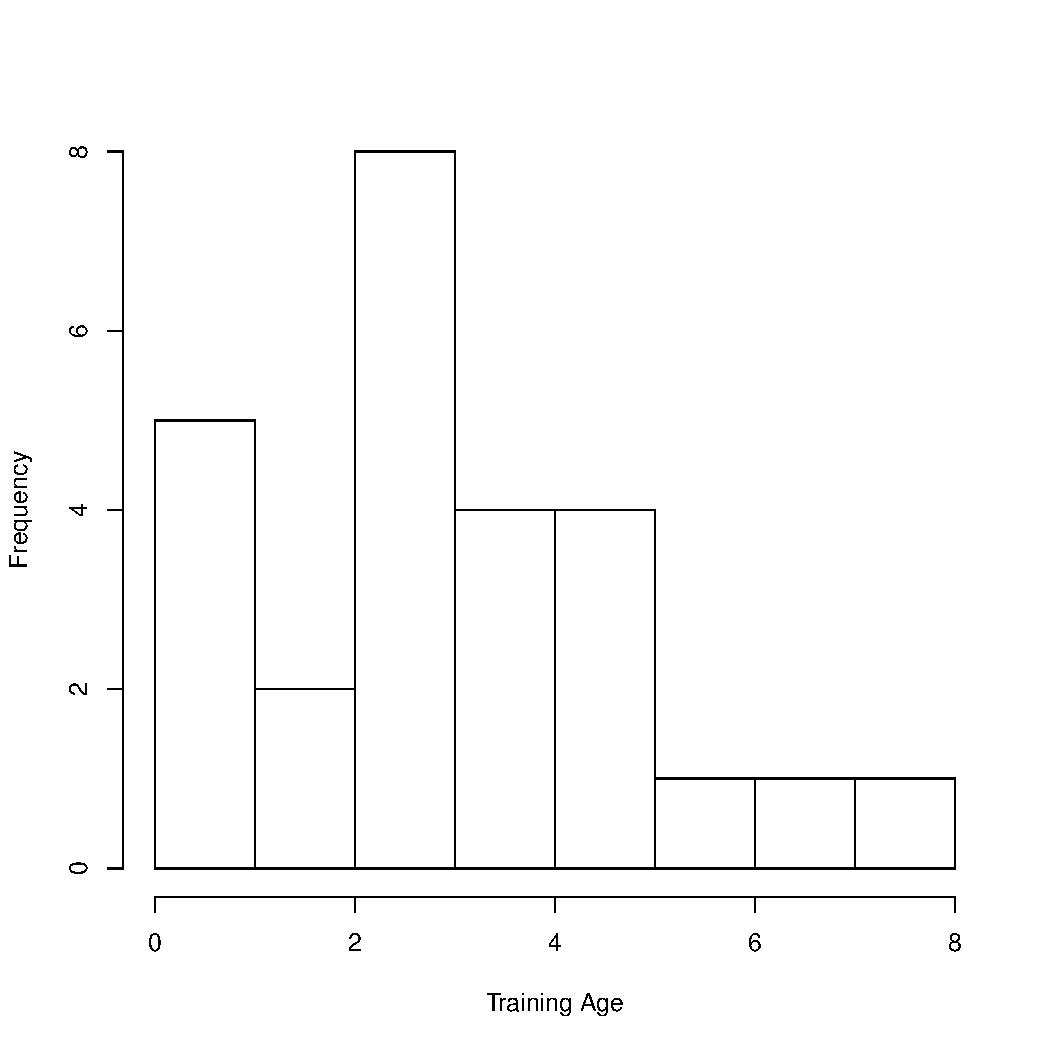
\includegraphics[scale=.3]{images/images/ethnoTrainingAgeHist.pdf}
       \caption{Distribution of athlete training age ($n = 26$)}
     \end{center}
       \label{fig:ethnoTrainingAgeHist}
    \end{figure}

18 of the 26 athletes had a background in other sports (16 athletes from track and field, one from football, one from basketball).  These athletes usually began part-time or full-time physical training at the age of 11 to 13.  Those who transferred to rugby from other sports did so either at the beginning of senior high school (16 years) or at university age (18 years).  The remaining eight athletes had no particular sporting background before rugby, and most began adherence to rugby at high school or university age (16---19 years).  These athletes were either scouted by the head coach of the rugby Program or by school athletics coaches based on their basic athletic attributes (running speed, strength, coordination, and potential for physical growth).\footnote{Of the 26 athletes in the squad, three junior athletes who were part of the squad when I arrived in September 2015 left before August 2016; and three new athletes arrived during the time I performed research.  This flux of athletes in and out of the team was quite common, due to the fact that recruitment often occurred informally via personal networks}.

The team consisted of 13 athletes who were considered ``senior athletes'' (\textit{lao duiyaun} 老队员).  Of these 13 athletes, eight athletes were considered part of the most senior ``starting team''
(one was a permanent employee (\textit{zhengshi} 正式)\footnote{Senior athlete Su Hailiang was the only permanent employee, by virtue of the fact that he was a Beijing resident.} and seven were full time contracted athletes (\textit{xieyi} 协议). The remaining five senior athletes were provisionally contracted on a ``training contract'' (\textit{shixun} 试训).  The remaining 13 athletes were considered ``junior athletes'' (\textit{nianqing duiyuan} 年轻队员). Six junior athletes were engaged by the Institute on ``student level'' contracts (\textit{erjiban} 二级班), and the remaining seven trained with the program on a ``trial'' basis (\textit{jixun} 集训); effectively on a trial arrangement until they showed promise or else withdrew from the squad).  Athletes contracted as students did not receive a salary but received in-kind support in the form of training, food, board, and health insurance at the Institute.  Most athletes were from urban and rural areas of northern China (Shandong (11), Beijing (6), Jiangsu (3), Liaoning (2), Hebei (2), Henan (1), Heilongjiang (1)).


\myparagraph{Expectations for athlete experience of uncertainty in group exercise}
Based on this information, I expected that, by and large, the joint action demands of rugby---particularly demands relating to team performance---will be a salient and observable feature of athlete experience.  Rugby is a minnow sport in China and athletes have very little recourse to familiarisation with rugby beyond spaces like the Institute. Thus, almost all athletes start from scratch with rugby when they arrive at the Institute (except for those athletes 5 who began training at another province or at the Chao Yang School, a school with a rugby program that feeds into the Institute).  Over half of the athlete cohort (15) had only three or less years of experience with rugby's joint action.  Five athletes were new arrivals, with less than one year of training experience, and only three athletes had greater than five years of experience.

High within-group variation athlete seniority and training age (denoting experience with the technical demands of the sport) should mean that variation in uncertainty will be more visible to observation: more senior athletes may appear more able to manage and mitigate uncertainty owing to higher levels of technical competence or familiarity; more junior athletes may appear more challenged by the uncertainty of joint action.

Rugby in China is thus a setting highly suited to testing research hypotheses formulated as part of a general account of team click in group exercise. In particular the mediating role of perceptions of team click in a relationship between perceptions of team performance and social bonding (Hypothesis 1), and the role of uncertainty in joint action in processes of expectation formation and violation, team click, and social bonding (Hypothesis 2).



\section{Coordination}


\myparagraph{On-field coordination}

Here, I report evidence to suggest that on field coordination in joint action was shaped by variation in technical competence and relational mode of social cognition promoting hierarchical relationism.  As predicted based on a consideration of rugby’s universally prescribed joint action demands, I observed that athletes engaged in high levels of interdependent on-field coordination of physical movement.  However, variation in technical competence meant that participation in on-field coordination was not consistent across all athletes.  The coach and senior athletes were heavily relied upon by more junior athletes to serve as directors of joint action.
E: Describing contours of cultural affordances (rugby, cultural, motivational) allows for vision of interdependence and coordination.

After a few weeks of observing training and a few sessions in which I myself took the team for training, the different factions in the team became quite clearly expressed on the field.  Generally speaking, the trialists were either on the sidelines learning and practicing the basics, or very tentatively beginning to join regular team drills in which all other athletes participated.  From my position of expertise it was clear to see that, of those athletes who trained regularly, the old-guard of Han Xiaolong and Lu Peng were the most experienced athletes.  Below them, the rest of the senior athletes varied in competence according to experience and individual differences, and student athletes from Chaoyang School were noticeably less experienced than their more senior counterparts.

The structure of training drills reflected constraints due to high within-group variation in technical competence.  Training drills were usually structured in such a way that athletes of similar abilities almost always trained together in the same subunits, rather than randomly assorting into subunits for each training drill (as was normal practice in rugby training sessions I had become accustomed to outside of China).  This tendency to group according to seniority and competence was most obvious in a basic passing drill involving four athletes per subunit (in which athletes would pass the ball between each other while running up and down the field.  Usually the most senior four athletes present at that training would naturally form the first subunit, followed by the next most senior (or competent), and so on, until the most junior and least competent or experienced athletes would form a subunit and attempt to emulate the preceding subunits.

When talking to senior players about this custom in training, I was told that the habit was necessary for two factors.  First, given that the differential in ability between the most senior and most junior athlete was so large, sorting according to seniority and competence (as opposed to randomly) ensured that the senior athletes could achieve a basic level of quality in their practice.  Second, by sorting together in sub units and doing the drill first, senior athletes could demonstrate the ideal standard for execution of each drill for the rest of the team to emulate.
E: Thus, on-field coordination in joint action appeared to be fundamentally constrained by within-group variation in athlete technical competence.

%hierarchical relationalism
After a few weeks of observing training I eventually began to coach the team myself, focussing on defence and ``contact'' work, and team play.\footnote{Contact refers to skills of rugby that involve body-on-body physical contact in addition to defence.}  For the first few weeks, athletes showed obvious dedication and conscientiousness when participating in training and learning the new content that I taught them.  One day approximately two weeks after I first started coaching the team,  I took a session in which for the first time almost all the senior athletes were unable to train, either due to injury or other commitments such as attending BSU for university matters.  The impact on the quality of training was palpable.  The junior athletes who were present were, for whatever reason, passive and unresponsive to instructions, and appeared unable to provide direction to the athletes below them.  Over time, a clear pattern emerged, in which the quality of training was more or less correlated with participation of senior athletes. Without senior athletes helping direct training, athletes---particularly the younger athletes---were generally slower to react to new information.  Often in such situations, more senior athletes who were present, would then usually become actively irritated by the poor quality of training, and begin to openly criticise the junior athletes.  This type of situation might be obvious and predictable in any team setting, and can probably be largely explained by stark within-group variation in technical competence.
E:

%\subsubsection{On-field hierarchy and structure to joint action}
 Athlete attitudes towards team performance revealed that perceptions of interdependence in on-field coordination were common and salient, albeit not always explicitly expressed. When talking to the senior athletes and coaches about the quality of training (or lack thereof), the most problematised of all the team factions was the group of ``training contract'' athletes, most of whom had just begun their undergraduate studies at BSU.  The basic consensus was that these undergrads lacked initiative and focus; they were too distracted by university, computer games, and pursuing romantic love. Having achieved the core goal of gaining access to university, the unruly undergrads were criticised for not possessing sufficient intrinsic motivation to dedicate them to rugby.

One day following a training session that I took, in which many senior athletes were absent, I walked back from the training pitch to the dormitory with assistant coach Shi and player-coach Han, and we began to discuss the issue.  Coach Shi postured his opinion on the situation:

        \begin{quote}
               Some athletes think its ok to just be an athlete here and get to BSU, and not pursue anything higher or anything more.  Actually, it's ok to think like that. But if that's the case then sorry, you'll have to watch from the sidelines.
           \end{quote}
          \begin{quote}
               有的球员觉得好在这当运动员上体大就可以了,不去追求更高的更多的。其实,可以这样想,但是,对不起,你要靠边看着。
           \end{quote}

%Shi's threat to sideline athletes for poor performance or focus was a relatively empty threat.  Usually coaches were desperate for as many athletes as possible to take the field to make up appro
Han offered a slightly different perspective, by explaining that he could see the reasons for the tendency for more junior athletes to lose focus. But he also insisted that, in the case of the beijing team, the undergrads were becoming habitually un-focussed during training:

         \begin{quote}
           It has become a habit.  When we were at CAU, at that time during university, we would also lack focus at times and so on, but back then, as soon as head Zheng would take training, we would all be immediately focussed!
          \end{quote}

          \begin{quote}
           成为一种惯性,我们在农大那个时候也会不关注等等,但是那个时候郑老师一带我们就全在关注
          \end{quote}

Coach Zheng was---at the time that Han was referring to---the most authoritative coach in Chinese rugby (see Chapter~\ref{sect:rugbyInChina}). The tales of Zheng's intensity as a coach were infamous (see Lu Peng's description of video analysis in Chapter~\ref{sect:openScrutiny}), and it was clear based on older athletes' recollections that Zheng's presence alone was enough to inccite deep anxiety-induced focus from athletes.
E:

Shi's explanation provided a rationale for a lack of focus at a more general level (i.e. on the level of general motivation for adherence to rugby).  It is conceivable that the structural incentives available for athletes would somehow impact on general motivation for adherence to rugby and its collective technical and social challenges.  Han's suggestion offered a more proximal explanation for athletes' lack of attention and focus in joint action on the field. In particular, the make-up of the group at training, including coaching staff, can have an impact on athlete's level of focus and attention.

%relating to the cultural terrain of rugby in China could offer affordances that enable and constrain certain patterns of social interaction and attention in joint action.

It was also possible top that both of these levels of explanation were subject to processes associated with a Chinese relational mode of social cognition.  Over an extended period of close observation, I could not help but develop the impression that---even after ``controlling'' for within-group variation in competence or utilitarian motivation for adherence to rugby, there was something related to the dominant habits and intuitions of social cognition generalisable to contemporary Chinese.  Considering existing evidence (outlined in Chapter~\ref{chap:researchSetting}) for the function of processes of hierarchical relationism in patterns of action and perception (as well as group formation and institutional norms), it is plausible to speculate that in a setting in which hierarchical relationism is most dominant as a mode of social cognition, the presence of figures of authority could be crucial for maintaining the quality of attention and focus in joint action.

Senior athlete Lu Peng, who had also been coached by Zheng Hongjun, tained an exchange that powerfully summarises the agency of the coach in directing behaviour in joint action.  At one point in the interview, we arrived at the conversation of the role of the coach in the team, particularly the idea that if athletes relied too much on the coach's direction it could be a detriment to team performance in joint action.  Lu reminisced on his time at CAU under the coaching of old Boss of the Beijing team and Chinese rugby, Zheng Hongjun:

          \begin{quote}
             ...one mistake or a bad decision, say if you didn't pass the ball when you should have, then you'd be taken off.  It doesn't matter how well you played before that, one basic mistake, for example, you were under a lot of pressure and you didn't judge the play properly, and you didn't pass the ball, but instead you took the ball forward, maintained possession...I don't think its such a big issue.
             Its not like we're talking about that type of situation where there is an obvious two-on-one scoring opportunity and you didn't pass the ball (to the open player)...
             But he (Zheng) won't accept it.  If you don't pass the ball (in that situation) he will yell at you, the pressure is extreme.  So we became very careful when we played, which developed a terrible habit, which was when---``baaang!''---you dropped the ball. When we made a mistake like that, we obviously knew ourselves that we had made a mistake.  But we'd still look to the coach first (so that he could confirm it for us)!!
               \end{quote}

               \begin{quote}
                    ...一点失误或者判断不好不传球就下来,你以前打的再好,一个简单的失误,比如说这个球压力很大。你在场上你美判断好,然后你没传,但是说我可以向前,保留球权,我觉得问题不是太大。
                   他并不是说想那种很明显的二打一机会我不传...
                    但是他不行,不传球就骂你,压力非常大, 我们打球的时候初伏小心。最后黑的什么习惯:“呗儿”(掉球)。。。 我们一失误了自己也知道失误。先看教练!
              \end{quote}
       E:

Conclude:
Inetrdependence of on-field joint action
Mediated by Competence,
motivation,
and hierarchical relationism.
E: an explanation of cultural terrain (affordances) allows for view of the salience of on-field coordination as a factor in athlete experience of joint action:
E: supports an investigation into instances in which this pathway ``clicks.''



\subsection{Social coordination}

Ethnographic evidence suggested that athletes' adherence to rugby was motivated by both utilitarian and social factors.  Most explicitly, athletes were motivated to commit to rugby for individual life-course opportunities of education and employment.  But, as became clearer to me through the process of extended observation, athletes also derived substantial social resources by virtue of their membership in the rugby team and the social coordination and interdependence that they shared with team mates, coaches, and the institute Leadership.
This evidence supports the suitability of rugby as a site in which to situate and test a theory of team click in group exercise.

After I completed each semi-structured interview, I asked each of the 26 athletes to complete an activity in which they were asked to rank (from most important to least important) their motivations for adherence to rugby at the Institute.  I selected these motivations based on preliminary unstructured interviews and conversations with athletes, coaches, and other knowledgeable observers.  The motivations included: ``Education'', ``For Beijing'', ``Family'', ``Gain Respect of Others'', ``For Teammates'', ``Employment'', ``Beijing Residency'', ``Money'', ``Enjoyment'', ``Popularity (with prospective romantic partner).'' I wrote each motivation down on a piece of paper and scattered them randomly on the surface of a table in my room where I conducted interviews.

Mean rank of motivations for adherence to rugby are reported in Table ~\ref{tab:athleteMotivations}.  It was telling to see that motivations of family and education ranked as the highest of athletes' motivations for rugby.  When asked in semi-structured interviews, almost all athletes agreed that their most prominent explicit motivation for playing rugby was to pursue life-course opportunities of education and employment.  Importantly, it was also commonly declared that achieving education and employment through commitment to rugby would make their families proud.

The fact that the opportunity for attaining tertiary education through rugby was more proximal to athletes than employment opportunities beyond university could perhaps explain the relatively lower average rank of employment. It was clear that most athletes were not immediately motivated by the promise of Beijing residency (perhaps because they deemed it no longer attainable).  In sum, athletes' motivations for adherence to rugby indicate that concerns for life-course opportunities and family were on average more dominant than motivations driven by team-based categories such as ``For Beijing'' or ``For Teammates.''  However, motivations derived from teammates or representing Beijing featured much higher than other motivations such as

    %\begin{table}
     % Please add the following required packages to your document preamble:
% \usepackage{booktabs}
\begin{table}[]
\centering
\begin{tabular}{@{}clc@{}}
\toprule
\textbf{Rank} & \multicolumn{1}{c}{\textbf{Motivation}} & \textbf{Mean (SD)} \\ \midrule
1             & Family                                  & 2.34 (2.35)        \\
	          &          	                            &        \\
2             & Education                               & 2.38 (2.19)        \\
	          &          	                            &        \\
3             & Respect                                 & 3.50 (2.61)        \\
	          &          	                            &        \\
4             & Represent Beijing                       & 3.58 (2.04)        \\
	          &          	                            &        \\
5             & Employment                              & 3.96 (2.04)        \\
	          &          	                            &        \\
6             & Teammates                               & 4.00 (1.94)        \\
	          &          	                            &        \\
7             & Enjoyment                               & 5.69 (3.16)        \\
	          &          	                            &        \\
8             & Money                                   & 5.85 (2.22)        \\
	          &          	                            &        \\
9             & Beijing residency                       & 6.42 (2.61)        \\
	          &          	                            &        \\
10            & Attract a partner                       & 8.00 (1.41)        \\ \bottomrule
\end{tabular}
\caption{Athlete motivations recorded following semi-structured interviews (n = 26)}
\label{tab:athleteMotivations}
\end{table}

     %\end{table}

As senior athlete Lu Peng explained to me in interview, for the prominence of education as a motivation for adherence to rugby:
        \begin{quote}
            Yeah,most of us in Shandong are like me, 80-90\% are of the same idea: there is an awareness that individual sports need less people, and so coming to rugby this type of team sport, most people’s goal is to use rugby to get to university.  But when I came to CAU I thought suddenly that I really like this sport, before I had never come into contact with a team sport before, and it was a team sport involving a ball, so I really liked it.
        \end{quote}
        \begin{quote}
             对,因为我们山东大部分人,都是像我这种,百分之八十到九十差不多都是这个思想,就是这么个意识就是说,单项需要人少,所以来橄榄球这类集体项目,大部分目的就是为了上个学。但是来到了农大之后我觉得我突然就喜欢这个项目,以前没接触过集体项目,而且有球的集体项目,所以我很喜欢。
        \end{quote}

In citing the obvious strategic motivation for adhering to rugby, Lu also admits that he immediately came to like and enjoy rugby once he began to train at CAU. I will discuss this common feature of athlete testimonies in more detail below. Here the main point is that the overriding motivation that lands athletes in rugby programs all over China is education first.

The fact that family was the highest ranked social category above team-related categories of ``For Beijing'' (4th) and ``For Teammates'' (6th) was indicative of the primacy of motivation related to immediate relational networks of each individual.  While representing Beijing was clearly important, and indeed rugby was the source of gaining respect from others (3rd), these motivations appeared to be coordinated by concerns primarily for family and life-course opportunities.  Very few athletes cited ``For Enjoyment'' (clear 7th) as the prime motivation for adherence to rugby.  It would not be inconceivable to see this as a strongly cited motivation for adherence to rugby in settings in which rugby exists as a popular mainstream sport.  Many, including some professional practitioners would claim to be adhering to a sport like rugby simply ``for the love of the game'' \citep{Jackson1998}.






In addition to athlete testimonies in interviews, I also witnessed a number of instances in which an athlete's mood fluctuated according to the state of their attempts to secure life-course opportunities of education and employment. Often the path to securing entrance to BSU was not always straightforward, even if athletes had earned the ``Master Sportsperson'' prerequisite.

Two senior athletes, Ma Haitao and Cui Suocheng, despite both long qualifying as Master Sportspersons, were involved in complex bureaucratic journeys in an attempt to gain admission to BSU.  One day early in my first stint of training I was taking a training session in which we were focussing on defence, and Shuocheng suddenly appeared to have given up all energy.  All of a sudden stopped doing the prescribed tackling drill.  I took him aside and began to take him through some of the details he missed last week when he was away.  He refused to listen and said, ``I get it, I just don’t want to do it, I’m sick of it, I’ve had enough of this drill'' (我知道怎么练,我就不想练了。练够了!)''You’ve had enough?'' I asked, ``Alright, if you’ve had enough then get off the field!'' (练够了?好吧,那你靠边去!).  I snapped at him, motioning to the stands for him to go and sit down. I was stunned that he first said that he didn’t want to practice. And then I was even more surprised when Shuocheng immediately followed my instruction and sat on a tackle bag on the side of the training field.  Later on in the training session, he came back over to the subsequent training drill and started offering (helpful) advice to the more junior athletes about their technique.

A few days later I found an opportunity on our way back from training to the dormitory to ask head coach Zhu about the situation with Shuocheng.  Zhu explained that Shuocheng was experiencing difficulty finalising his contract transfer from Shandong to Beijing province, and that this procedure was interrupting his ability to process his university application (Shuocheng had moved from Shandong provincial team in 2014). To attain prized life-course opportunities through adherence to rugby was obviously a core motivation for most athletes. At times for some, the issue became critical enough to seriously these impact on athletes' on-field performance.

Ma Haitao, another senior athlete also in the process of trying to apply for university (after years of delays), also experienced large amounts of stress during my time researching.  One day he spoke to me at length about the way in which these difficulties were impacting on his mood and his ability to focus on training. ``It impacts me so strongly'' (对我的影响太厉害了) he said as we walked to the canteen after a training session. ``I’ll probably need to have a long sleep or take a break from training before I can recover from these sort of frustrations---the endless process of getting this form and completing that form, its so frustrating'' (我可能要先睡个好觉请假休息才能回复过来呢。这个那个证,跑断腿盖章了,令人太沮丧了.)
E:


\myparagraph{Institute as platform for the interests of an hierarchical relational network}

At times during my research it appeared that the rugby team and the Institute were overtly coopted as a platform for certain authoritative individuals to pursue strategic motivations, namely the pursuit of education opportunities.

A powerful example came one week before the the final National Championship Tournament in July 2016 (the Tournament during which I performed the survey study (Chapter ~\ref{chap:trainingExperiment}), a very large and overweight young man appeared at training.  He did not appear to display any direct athletic potential relevant to rugby (he was quite heavy-set and physically undeveloped), and it was also clear that he completely unfamiliar with rugby.  I was somewhat puzzled by this new arrival.

The only other analogous situation I had previously witnessed was occasional coming and going of the son of Vice-Principal Wang. Wang's son, known affectionately as ``Chubs'' (小胖), was a normal (non-athlete) student at a local Beijing high school student.  Chubs had no specific background in sport, but would join the team's training during sessions during periods in which his school was on holiday break.  Chubs had become a popular and welcomed presence in the team; he assumed the role of most junior member of the team and diligently performed all the tasks expected of him in this role (carrying training gear to training, filling water bottles, etc.). He was gregarious and always positive in public situation, and was willing to embrace the many foreign and intimidating skills associated with rugby. Indeed, over time training with the team, Chubs became considerably less physically chubby, and more and more competent in rugby.

Originally I had not thought too much about Chubbsy's motivations for adherence to rugby during school holidays.  I assumed, perhaps somewhat naively in hindsight, that the vice-principal wanted his son to participate in a team sport which had many positive educational and health benefits.  I was forced to rethink this assumption once I discovered the reason for this newest arrival less than one week before the year's most important Tournament.  As coach Wang later explained to me, this young man was also a local Beijing high school student and was also related---in some more or less direct way---to a different vice-principal at the Institute (Wang didn't specify exactly who, apart from referring to them simply as a ``Leader'' (领导)).  Wang explained to me that this new arrival needed to quickly familiarise himself with rugby, because he was to be named in the Beijing team for the weekend's Tournament.  At some point during the Tournament, he was going to take the field, and in so doing, attain the athlete qualification standard of a ``Master Sportsperson''  This qualification would enable him to attend the prestigious BSU through the athlete pathway.

This scenario chafed against all of my intuitions about rugby and institutions.  My many years spent playing team sports and absorbing egalitarian and meritocratic cultural narratives common to Western democracies and particularly to my homeland of Australia---the land of the ``fair go'' and the ``tall poppy syndrome.''  Here, a young, roughly 17 year old overweight student with no athletic ability and no familiarity with the game of rugby was planning (under the will and organisation of the those who wielded power in his relational network) to take one of the 12 positions available to the Beijing team and play his first (and probably only ever) game of rugby so that he could take the field and therefore receive a passage to a prestigious university.

``The Leader has the final say, I can't do anything about it'' (领导说的算,我没办法)said head coach Wang, helplessly, when I pressed him on it.  At the time, Wang was only half way through his first year as head coach.  It was possible that he had been targeted as a coach who could be manipulated.  Indeed, it was quite possible that rugby more generally had been identified as a sport in which these types of activities were permissible, or possible without raising many eyebrows beyond those of the Australian anthropologist on the sidelines of an empty stadium at the National Tournament.

E:

This was an instance when the power enacted in the relational network was more dominant than the power of the social institution in which these hierarchically structured relationship were allowed to take place.  The categories of the team and the Institute held less sanctimony than the imperative of regulating and harmonising relationships in a hierarchical network demanded more attention.

Instances such as this one demonstrate that the relational mode of interacting captures attention and perception. Any sanctity around the institutional boundaries of the team or the Institute appears to be secondary to activity that appears on the surface to be purely strategic, but in reality stems from a deeply relational social logic to the research setting.


E: As I came to understand, these processses were not purely utilitarian, but activated a social logic of hierarchical relationism



The relatively sudden change in head coach half way through my first stint of ethnographic research gave me the fortunate opportunity to witness the implications of this transition for the social organisation of the team.

When I returned to Beijing after a 10 day travel break in February, almost a month after head coach Wang had replaced former head coach Zhu, two of the athletes who were on trial under Zhu's tenure---Xu Gong and Lian Jianxiang---had since left.  When I asked senior athlete Wang Wei about the disappearance of these two students, he suggested that ``they had interests with Old Zhu...Old Zhu said that he could solve their ``school problems'' [i.e. get them into university]. They were here to try to get in to University.'' (和老朱有利益关系,老朱说可以解决上学的问题 都是过来上学的).
%Talk of arrangements of this nature in sport was hushed but common, and it came as no real surprise to me by that stage that there may have been

In fact, my question to Wang Wei that day was in part prompted by the fact that a group of four new trial athletes had just arrived from a high school in the neighbouring province of Hebei.  Apparently, someone in Wang's relational network had introduced these athletes to Wang, and they arrived at the Institute and joined in training for the day.  This coincidence was a telling indication of the power of the coach to coordinate the members and activities of the team.  The Institute and the team serve as platforms for activates of relational networks to unfold.  An athlete is only categorically related to the team by virtue of his or her capacity to adequately participate in and foster social relationships that play out on that institutional platform.  In this research setting, I found evidence that social categories of team and Institute served less as sanctimonious categories for social identity formation, and more as platforms for opportunity and advancement through regulation and harmonisation of relational networks.

I began to realise that individuals who occupied higher positions had considerable power to influence the social activity that unfolded in the institutions of the Institute and the rugby team within the Institute.   The head coach, for example, appeared to be very influential in deciding which athletes could participate in the team.  The change in head coach half way through my first stint of ethnographic research gave me the fortunate opportunity to witness the implications of this transition for the social organisation of the team.

%\subsubsection{Leaders have the final say\label{sect:leadersFinalSay}}

E: Understanding of relational mode of social cog important to identity (to avoid misapprehension, e.g. utilitarian motivations purely).
E: Allows to glimpse the structure and contours of the social interdependence and coordination associated with rugby at the institute---> ultimately affordances that bear upon actions and perceptions such as team click.











\subsubsection{``I have become a social animal''\label{sect:socialAnimal}}
Despite clear utilitarian motives for adherence to rugby, athletes nonetheless also experience strong perceptions characteristic of social bonding.  While the Institute was not the traditional social rugby club or school team found in England or New Zealand, athletes  did live, eat, and sleep together, some spent the majority of their formative high school, university, and young-adult years together playing rugby.  Thus, the interdependent nature of rugby promoted processes characteristic of social bonding that athletes were unable to avoid.

As foreshadowed by Lu's comments in interview above, enjoyment of rugby was a recurrent theme when asking athletes during interview about their motivations for adherence to the sport.  Athletes suggested that rugby was either fun (\textit{haowan} 好玩), interesting (\textit{youyisi} 有意思), fresh (\textit{xinxian} 新鲜) or stimulating (\textit{ciji} 刺激).  Often, as was the case with Lu, declarations of enjoyment were often accompanied by citations of more obvious incentives relating to the pursuit of tertiary education.

  As Big Mouth Lu explained:
            \begin{quote}
                At the time, I stayed here (to play rugby) for two reasons.  The first was that I thought this sport was really enjoyable. The second was also rather precise, one really important thing that came to me was that coach Zheng Hongjun assured me that he would solve my schooling problem, and so then I decided to stay here.
              \end{quote}
             \begin{quote}
                 当时留下来有两方面的原因,第一是我觉得这个东西很好玩。第二也是算很确切的,很重要的一个东西涌向我就是,郑教练给我保证说会给我解决上学的问题,然后就决定呆在这里了。
               \end{quote}

Ming Xiaokai offered a similar rationale, citing education first, and enjoyment of the sport as a secondary motivation.  When I asked him what his parents thought of him playing rugby, he explained:

        \begin{quote}
          They (my parents) don't have many thoughts about it, because they think me making it in to university is already fantastic! I am now already at university (at BSU), but I play it [rugby] because I really like it, I still want to keep developing with it. Before it was for getting in to university, after making it to university now I want to train hard, now I really want to develop this thing.
          \end{quote}
        \begin{quote}
           他们没有什么太大的想法。因为他们想我考上大学已经不错了!我现在已经上大学了(体大),但是我是喜欢这个东西才还练,我还希望在往上走一走...之前为了上大学,上大学之后就想好好练,现在就想好好发展这个东西。
         \end{quote}

Lian Jianxiang also felt compelled to yoke enjoyment to his rationale about pursuing rugby for the purposes of education:
               \begin{quote}
                       Before I wanted to go to university there (at my old school), but I didn't get in.  Then I heard there was this program here, I really liked rugby, but my province didn't have this sport. At the time my coach said that there was this opportunity, if you play rugby you'll be able to get into university.  And so I wanted to come and give it a try, and as a result I've been here until now.  I really like (rugby).
               \end{quote}
               \begin{quote}
                   我之前在那想考学,但没考上。后来听说有这个项目,我挺喜欢这个项目的,但是我们当时省里没有这个项目。当时(教练)说这有个机会,练橄榄球就有机会上学。我就想来试试,结果就一直到现在。挺喜欢.
               \end{quote}

Reading these rationales on the page may encourage the interpretation that athletes were deliberately citing enjoyment for rugby as a deliberate strategy to disguise the clear utilitarian motivations behind their adherence to the sport.  When conducting interviews, it did not appear to me that athletes were deliberately or forcibly including enjoyment as a rationale for adherence to rugby.  Instead, the enjoyment came across as genuine—--perhaps due to the honest surprise with which athletes realised that they had come to enjoy rugby (contrary to prior expectations).

It was clear that life course opportunities motivated athletes' initial journey to the Institute.  But upon arrival, athletes became completely immersed the life of the team, and the psychophysiological demands of this immersion were all encompassing.  For most new recruits, while rugby was technically challenging and socially complex compared to the individual sports (or non-sporting backgrounds) from which they had transferred, rugby was also new, stimulating, and interesting.

Senior athlete Wang Wei explains that his identification with rugby was a gradual process of familiarisation. Once familiarised, however, Wang came to like the sport in an irreversible sense:
             \begin{quote}
               I guess its exposure, when I first started my first impression was that it was barbaric, then after that slowly after more exposure to rugby I thought that this sport is really suited to males, I thought that this sport is a really good sport, I thought I had gradually come to like this sport.  At the beginning I thought it was too barbaric and wasn’t game to play, not game to tackle anyone to the ground or whatever, but after I’d been exposed to it for a long time, I came to understand the culture, and I came to like the sport.
           \end{quote}

             \begin{quote}
               还是接触吧,刚开始第一印象觉得野蛮,后来慢慢接触之后觉得这个项目挺适合男性运动,觉得这项目是个挺好的项目,觉得自己后来慢慢喜欢这个项目了。开始的时候觉得野蛮不敢打,不敢扑倒什么的,后来接触的时间长,了解这个文化了,就喜欢上这个东西了.
             \end{quote}

    Many more senior athletes explained that their experience of rugby had developed beyond surface interest and enjoyment, to a more substantial and irreversible processes of social and psychological attachment.

    As Ming Xiaokai continued to explain to me (following on from his comments immediately above):how they became to develop a level of irreversible attachment to rugby and the social resources that it offered:

           \begin{quote}
               Before it was all for getting into university, now that I'm at university I think its really good, I can't let go of it.
               I only learnt about rugby after I came to the Institute, when I here training for athletics.  I have been playing rugby for just on two years now, before that I was doing 100m in athletics.  Right at the start I found it hard to accept, I didn’t really like it. Now I think I already have that feeling where I can’t leave.  I’ve now had that time to understand it, I now like this sport, but I’m still really really poor at it.
           \end{quote}

           \begin{quote}
               之前是为了上大学,上大学以后的感觉挺好的,放不下。我是来先农坛之后认识橄榄球的,我之前是练田径的。打橄榄球刚两年,之前是百米田径。刚开始很难接受,不太喜欢,现在觉得已经有点离不开的感觉了。有了这个理解的时间,喜欢这个项目,但是练得还是差很多很多.
           \end{quote}

Xiaokai expresses something of a middle ground in relation to social identity derived from adherence to rugby.  After approximately two years of training, Xiaokai found himself at a point where he is neither certain about his goals beyond attending university, nor is he able to imagine doing anything else---he is thus by default attached to rugby, by virtue of the path dependency of his progression through life.

Beyond explicit declarations recorded in interview settings, athletes' identification with the team and with rugby was evident from their use of other communication platforms.  Social media, for example, was a highly visible forum in which athletes would signal their social identity to friends and family.  Both junior and senior would display their connection to rugby on their individual WeChat accounts, by either changing their alias to include some reference to ``rugby'' or their profile picture, to display a photo of a rugby ball or a famous rugby player (see Figure ~\ref{fig:bjmWeChatProfile}).

         \begin{figure}[htbp]
           \begin{center}
             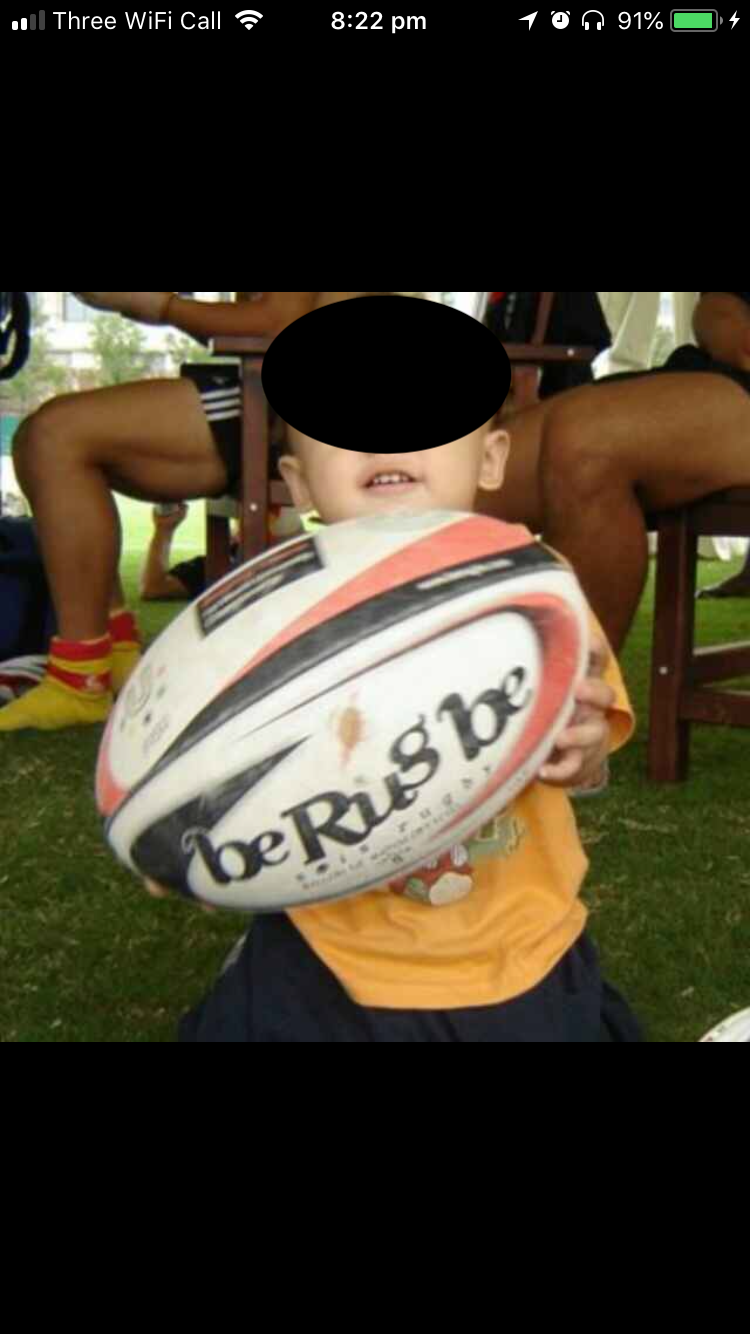
\includegraphics[scale =.1]{images/bjmWeChatProfile1.png}
             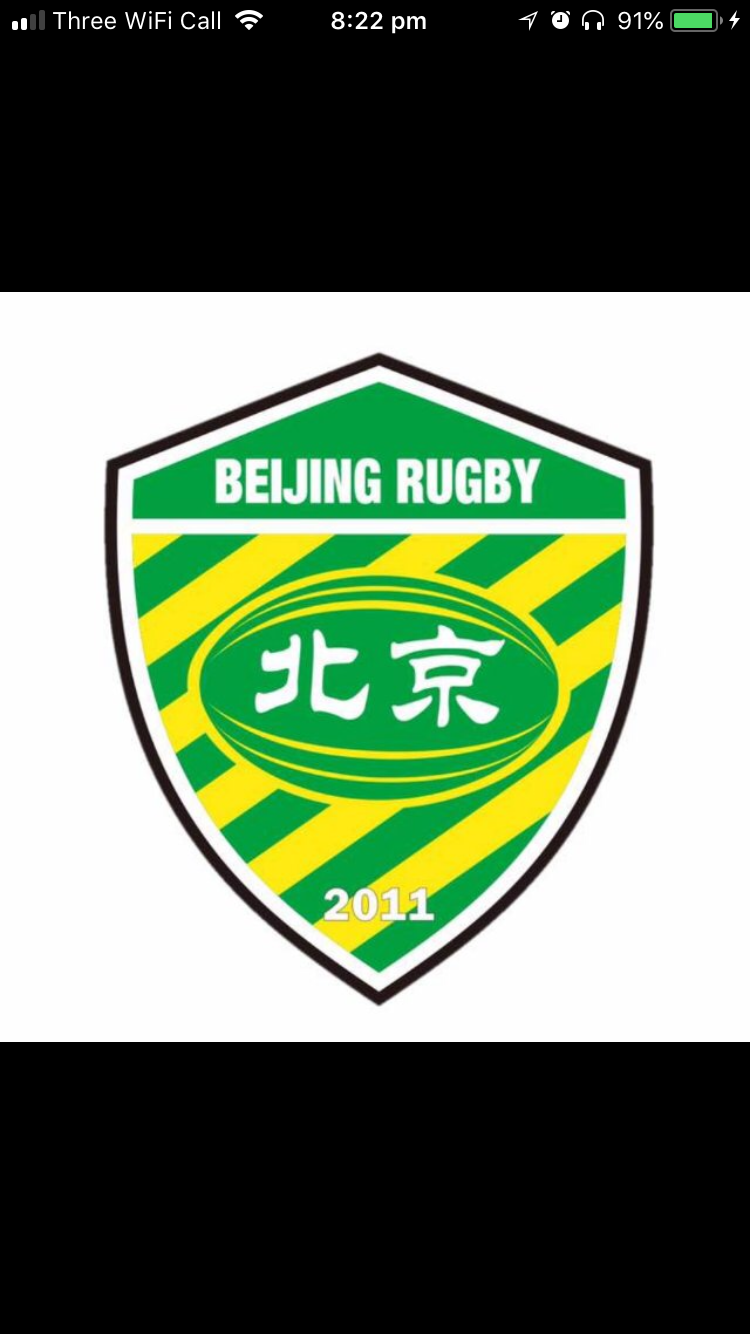
\includegraphics[scale =.1]{images/bjmWeChatProfile2.png}
             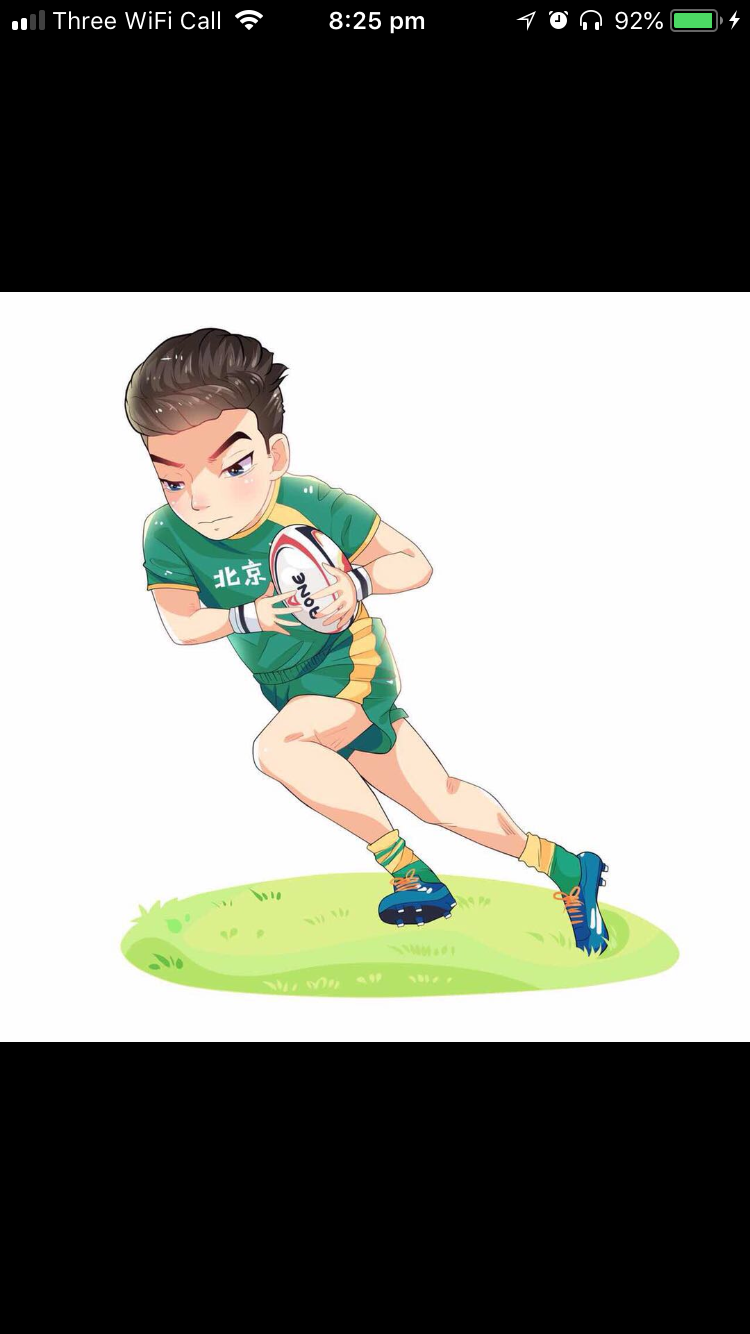
\includegraphics[scale =.1]{images/bjmWeChatProfile3.png}
             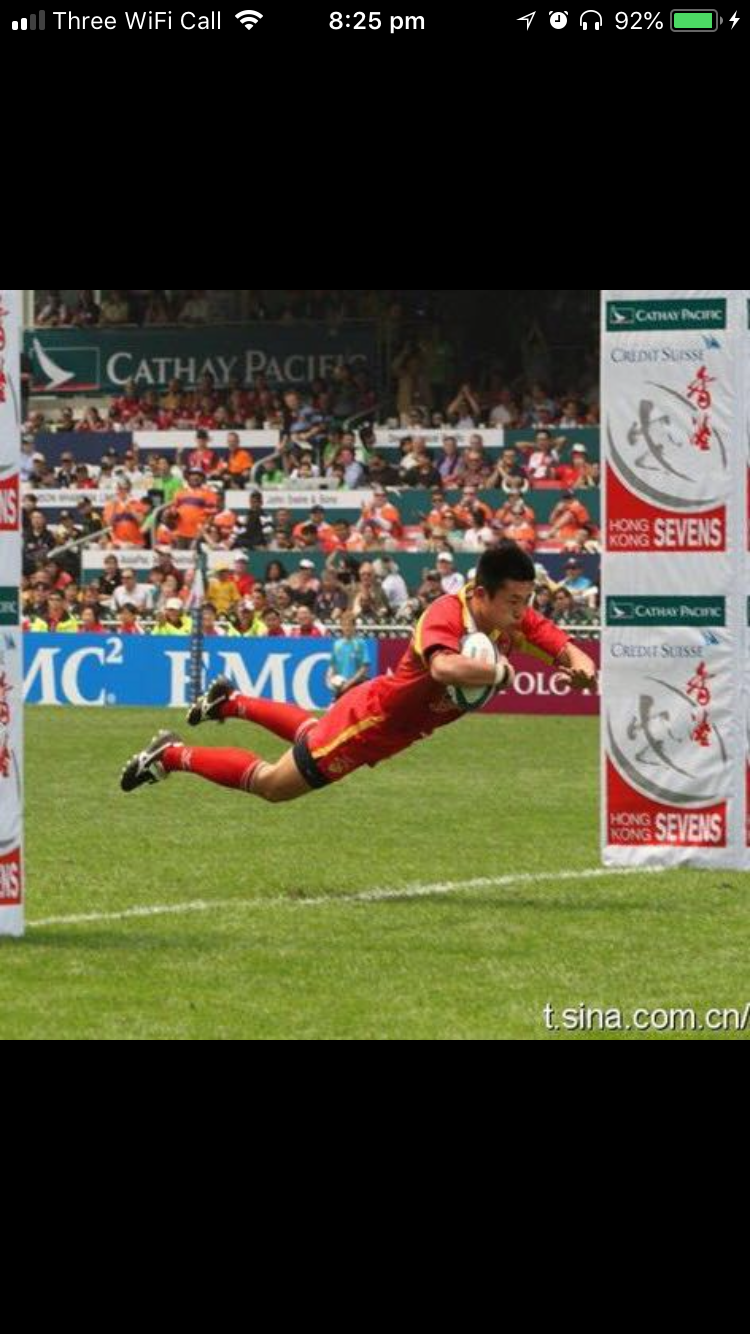
\includegraphics[scale =.1]{images/bjmWeChatProfile4.png}
             \caption{Screen shots taken from the social media profiles of a selection of athletes}
           \end{center}
             \label{fig:bjmWeChatProfile}
         \end{figure}

         %\myparagraph{Signalling on social media}
Athletes commented to me that the rugby team at the Institute used to be the most formidable and successful team in the Institute, and that despite the recent fall from grace, the rugby team were still highly revered by the rest of the athletes at the Institute.  In the activity survey of motivations for adherence to rugby administered following semi-structured interviews (see Chapter ~\ref{chap:ethnoField} Section ~\ref{sect:athleteMotivation}), athletes on average cited ``to represent Beijing'' as their 4th highest ranked motivation for adherence to rugby, one spot below ``to gain respect.''  Both of these motivations show that adherence to rugby offers considerable social identity resources.

Ma Haitao explained to me the development of his feelings of belonging to the team:

             \begin{quote}
               When I first came my sense of belonging was not strong, in terms of joining the Beijing team, because I didn’t have anything, I couldn’t play! I wasn’t playing with the team, I wasn’t anything.  At the time in my heart I felt, being a Beijing Team member means going out and representing Beijing in a tournament.  If you haven’t represented Beijing then I felt like I hadn’t made a contribution, I could say to myself that I was part of the team, but I couldn’t actually recognise myself as being part of the Beijing team.  Now, last year when I played in a tournament, now I have that recognition. ``Are you in the Beijing team? Have you played in a tournament?'' (If the answer to these questions is) no, then I don’t recognise it myself.  Only last year after playing a Tournament did I slowly start recognising that I was part of Beijing team.
             \end{quote}

             \begin{quote}
               刚来的时候归属感不强,就加入北京队,因为什么都没有,啥都不会,没跟着一块打球,什么都不是。当时心里觉得什么是北京队,就是出去代表北京队比赛。没代表北京队就感觉自己也没为北京队做过贡献,说自己是北京队,自己都不认可自己是北京的。现在去年打比赛了,才对自己有认可。“你是北京队么?比过赛么?”没有。自己不认可。去年打完比赛才慢慢开始自己认可.
             \end{quote}
Ma explains that his ability to equate his personal identity with that of the Beijing team was contingent on him representing Beijing in national tournaments---before doing so he ``was nothing.''  This passage is a great demonstration of the power of the team as a coordinator and administrator of social identity.  It is interesting to note that for Ma, concrete on-field actions (taking the field for Beijing) signal authentic group membership.  Without the proven technical competence required to take the field for Beijing in a national tournament, Ma was unable to subscribe to Beijing rugby as a core personal identity. Social identity dependent on on-field performance.


\subsubsection{Interdependence}

Recognised that a large part of the attachment involved interdependence with others:
   Wang Zhankun, a junior athlete and young hopeful of Chaoyang school, provided the following response when I asked him what he had learned from transitioning from an individual sport to a team sport:
         \begin{quote}
           Unity: seven people bound together.  Not like in an individual sport, where you’re just one person. In a team sport you must have seven people with one heart, you know, play against them with one heart.  If you have one who is not on board then you’re whole team is no good.
         \end{quote}
         \begin{quote}
           团结,七个人绑在一块,不像个人项目,就自己一个人,团体就必须得七个人同心嘛,同心和他们打。有一个不同心你整个不行。
         \end{quote}

\subsubsection{Team}
The concept of ``team'' (\textit{tuandui} 团队) was highly salient in group discourse, and it offered a (new) concept used to capture the interdependence.  Sun Hongwei's description of the team (reported in the introductory vignette to Chapter ~\ref{chap:theory}) offers a similar exposition of the novelty of the team dimension of rugby. When I asked athletes what new things they had learnt from rugby, an overwhelming response was ``team awareness'' (团队意识), ``team spirit'' (\textit{tuandui jingshen} 团队精神), and ``team work'' (\textit{tuandui peihe} 团队配合) were commonly invoked as ideal ethics of group membership for the rugby team.

During the course of semi-structured interviews, it soon became obvious that the concept of membership to an abstract category such as a sporting ``team'' was not indigenous to most athletes' experience before arriving at the Institute to play rugby.  Guo Junping, the youngest and most recent of the arrivals to the program during my time conducting research, had very little to say during our interview. He did however comment enthusiastically on the novelty of ``team'':

\begin{quote}
  It was only when I started playing rugby that I knew what a team was, before when training for athletics (everyone) liked to do it on your own!
\end{quote}
\begin{quote}
  练的时候才知道团队,以前练田径的时候都喜欢自己一个人单干!
\end{quote}

Lian Jianxiang, a young trialist at the Institute (the athlete who was relationally connected to Coach Zhu, went into more detail:
       \begin{quote}
           Before I wasn’t used to it, and then later as began to interact with my senior teammates, I discovered that it was more or less the same as my previous (athletics) team, but just more cohesive.  But there was still a difference, for example in an individual sport you need to manage yourself and that's all, whereas team sports you need to consider more, you need to consider a lot of things that relate to everyone...[By now] I am used to it. I like this feeling [of team sport membership] more, its so much better than individual sport, in an individual sport its just yourself, its too independent. This (rugby) is a big family, isn’t it?
       \end{quote}
       \begin{quote}
              之前不适应,后来和师兄一接触发现和我之前的队也差不多,要团结。但还是有差别的比如说之前个人项目管好自己就行了,团体项目考虑的比较多,要考虑好多大家一起的东西...习惯了。更喜欢这个感觉,比个人好太多了,个人只不过自己,个人项目太独立了,这个是个大家么 \\
        \end{quote}

   Unruly undergrad Fang Chao explains how he was transformed by rugby and the team:

       \begin{quote}
             I think before when I was doing athletics, compared to now, I think I am no longer the same person.  When I first came into contact with rugby, before I was doing an individual sport.  Now this is a team sport. I've changed a lot in terms of my personality, before when doing athletics I thought I was very independent and self-reliant, my own person.  Now I am one person who needs to communicate a lot with other people, cooperate; I have become a social animal.
       \end{quote}
        \begin{quote}
             我觉得之前练田径,跟现在橄榄球比,觉得我完全不是同一个人了。橄榄球刚开始接触的时候,之前田径是个人项目,现在是团队项目。性格方便改变很多,之前练田径是觉得我是个我行我素,自己一个人,现在我一个人还需要和别人多沟通,合作,变成群恤动物。
       \end{quote}
       E: For the majority of athletes who came from the individual sport of athletics (and the athletes with no prior team sport background), the team dimension of rugby was a distinctly novel experience, involving a suite of new social norms and requirements associated with group membership.



\subsubsection{Family}
The concept of ``family'' was central to the rugby program's public discourses surrounding social norms of group membership.  From vice-principal Jenny, through to the head coaches, and the athletes themselves, family was the metaphor most commonly used to convey the requirements of each athlete in-group.

The prominence of conventions associated with family were identifiable in the naming conventions of the team.  As a general rule, when directly addressing elder athletes, an athlete would add the suffix ``\textit{ge}'' (哥) to the elder athlete's first or last name, to indicate that the elder athlete was relationally equivalent to an elder brother.  When addressing Han Xiaolong, the most senior athlete in the group, for example, athletes would commonly use \textit{Long Ge} (龙哥).  When referring to the coach, on the other hand, athletes would use either the formal and respectful ``Teacher'' (\textit{Laoshi} 老师), ``Coach'' (\textit{jiaolian} 教练), or the more colloquial suffix abbreviation of \textit{dao} (导). The naming conventions for the coach derived from a Confucian tradition of master-apprentice relationships---originally structured on familial relationship conventions \citep{Spence1999}. When referring to a teammate in the third person, athletes would often refer to them as either their senior apprentice \textit{Shige} (师哥) or junior apprentice \textit{Shidi}(师弟), depending on whether the teammate was older or younger.  The network of relationships of the rugby team were thus modelled using hierarchical familial and Confucian master-apprentice relational conventions.

The metaphor of family contained room for expressing both the solidarity and emotional support of shared membership, as well as a justification for the hierarchical structure of the group.  Senior athlete Wang Wei offered his perspective on the family-like structure of the rugby program at the Institute:
    \begin{quote}
      Its not as if there was not a lot of new stuff, because I guess at the time I was playing basketball---basketball is also a team sport.  But the only little bit that rugby made me experience was respect for elders, newcomers must respect senior team members, senior members must take care of junior team members, this is something that I didn’t experience in basketball.  At the time also I didn’t understand that much, I guess China has always had respect for elders, but it didn’t come up for me in basketball, and so then when I came to rugby my experience of it was very deep.
    \end{quote}
    \begin{quote}
       那倒没有很多,因为我当时打篮球嘛。篮球也是集体项目但是唯一一点和橄榄球比让我体会到就是长幼尊卑,新人得尊重老队员,老队员得关照小队员,这是我在篮球上面没体会过的。当时也没了解这么多,中国文化一直有尊老爱幼嘛,在篮球队没体现过,然后到橄榄球队还是体验特深的。
    \end{quote}

Wang Wei first arrived at the Institute in 2011, during a time when the range in ages of athletes at the program would have been quite extreme, with the youngest athletes being around 16 years old, and the oldest athletes being in their mid 30s (the age range of athletes during my research was 15-28 years).  In this sense, it can be inferred that the conventions associated with family in China functioned as a resource that enabled Wang Wei to navigate the social terrain of group membership.  Affordance of family offered a way to deal with large variation in experience and familiarity




\subsubsection{The entire system must be aligned \label{sect:systemAligned}}

At times the more relational quality of social interdependence was revealed to me. I encountered a number of instances in which it appeared that athletes perceived their social domain to extend well beyond the interplay of immediate social categories of self and the group.  Instead, categories of identification were more porous, and what was more essential was an higher levels of coordination or alignment between key elements of the social system, especially those more senior in the hierarchy.

One example occurred the first morning I arrived back for the second major stint of ethnography in the summer of 2016.  I arrived back to a terrible incident in which some of the rugby team had been effectively poisoned accidentally by pesticide sprayed on the hedges outside their dormitory windows.  A few days before I arrived back, the groundskeepers had carelessly sprayed pesticide on the hedges outside the windows of the bottom-floor dormitory rooms of which the rugby team were inhabitants.  Some of the pesticide had made it in to the rooms of the athletes via open windows, and had caused a few of the athletes to develop throat irritations and coughs.

Senior athlete Wei Wenxin, who replaced Han Xiaolong as team captain after Han was promoted to assistant coach following the change in head coach in January 2016), was one of the most seriously affected by the pesticide, and when I sat down with him at breakfast the first day I returned, he explained the story with deep anger and outrage.  Importantly, when I asked him what was going to happen with all of this, he said to me ``the Leadership will have to say something about this, we are all waiting to see how Leadership will respond.'' (领导们必须要说话,我们在看领导们怎么说).  I found it interesting that Wei was so emphatic about the primary role Leadership ought to play in adjudicating this matter.  The role of political leadership in an organisation such as the Institute was no doubt crucially important to manage such issues, but the fact that Wei was so emotional and emphatic about this fact---almost as if the Leadership had a paternal role to play---was revealing of the emphasis Wei placed on an the need for alignment between levels of the social system in which he was situated.

My close interactions with the coaching staff confirmed the importance of hierarchical interdependence. During my second extended period of ethnographic research, which was well into the transition from head coach Zhu to head coach Wang, I shared a dormitory room with head Coach Wang's offsider, assistant coach Zhu Jing.  Zhu Jing had recently arrived from the rugby program at Xingjiang province, after Wang invited Zhu to join him as assistant coach.   Wang needed Zhu for support: to be his loyal leftenant, and to lighten the load on player-coaches Han and Lu. Despite transitioning to the official position of coach, Han and Lu were still required to train and play, at least until the National Games in 2017.

Zhu Jing was a new arrival to the team, and was thus on unstable ground. At the time he had no official contractual relationship with the Institute, and his position was therefore tenuous and contingent on his relationship with head coach Wang.  Zhu was neither a particularly celebrated rugby player during his time as an athlete at CAU, nor was he a particularly experienced or successful coach.  What he did posses, however, was a close relationship to Wang (they were classmates at CAU). Zhu was valuable to Wang for his loyalty---useful to Wang in his attempt to stabilise his leadership of the team---an inherently slippery platform for social activity (see Section ~\ref{}). In terms of his value to the team as a rugby coach and the Institute, however, Zhu still had much to prove.  If I were in his position, I thought, I would have done everything possible to help head coach Wang and the team—understood as  a category demarcating the athletes and coaches only---to improve performance.  As part of this, no doubt, I would seek to signal diligence and commitment in the way I went about my business as a coach.

After about two or three weeks into our roommate relationship, it became clear to me that Zhu Jing was not so concerned with signalling diligence, at least not to me, and not to the athletes either, at least not in a way that I personally recognised.  Most mornings I would wake up at 7:00am to attend breakfast with the athletes and then collate my field notes and prepare for morning training, starting at 9:00am.  Zhu, on the other hand, would reliably sleep through until roughly 8:50am each morning, and then turn up to training usually at around 9:20am after athletes had completed their warm up.  After lunch, Zhu would return to bed, usually from 1:30pm until 3:00pm, depending on when afternoon training was scheduled.  Afternoon siestas are admittedly an institutional in China's work life, but routine indulgence in a two-hour nap was surely taking the institution to its extreme.  I rarely witnessed Zhu spend any time working on preparing training schedules or other forms of professional development.

As it turned out, head coach Wang also began to notice the way in which Zhu was approaching to his job.  After the final Tournament in Qian An in July 2016, the team went out together for dinner.  This dinner was much less ritualised than the first team dinner organised by Wang earlier that year.  This time,  junior athletes were in one room, and the senior athletes and coaches were in another room, free to socialise within their more naturally occurring social factions.  Towards the end of the evening, after the effects of alcohol had well and truly set in, a heated discussion developed between head coach Wang and assistant coach Zhu. The discussion began with one of Wang's numerous toasts to the group at the table.  Wang said that it was important that the rugby program distinguished itself as an excellent team at the Institute, and there was a need for all senior members of the team (seated at the table) to contribute to this project.  It became clear that Wang wished to emphasise the need for Zhu in particular to ``lift his game'' in this regard. Wang explained that as head coach he was burdened with a lot of administrative work that detracted from his ability to manage athletes and training.  Given that the team was without a dedicated team manager (who would usually manage daily concerns of athletes and organise team logistics), Wang suggested that Zhu ought to improve his contribution. ``As an assistant coach, you need to conduct yourself at a high standard'' (当助理教练你要作为一个高度) said Wang directly to Zhu, indicating that his current standard was not acceptable. Wang spoke politely, but the public nature of these remarks suggested that he was using the opportunity to formally criticise Zhu.

Zhu retorted defiantly, directing attention away from his personal standards to the global situation of the team at the Institute.  Zhu suggested that the most important thing was that the leadership of the program supported the program, and only then could the program achieve a high standard: ``you have to have the support of leadership'' (必须有领导的支持).  Lu and Han, the next most senior team members present, also became involved in the discussion, with Lu siding more with Zhu and Han siding more with Wang.

The next morning, Zhu and I lay in our dormitory room beds, hung-over from ceremonial drinking after the team dinner the night before.  Zhu revived the dinner incident with me, seeking my support for his position.  Zhu insisted that his ability as an individual was fundamentally limited if the Leadership did not appear to offer him support.  I was in no state to record or write down Zhu's remarks, but his message was clear. If the team does not have the faith and support from the Institute (which in this case, it clearly did not have, at least since 2013), then how was Zhu supposed to perform his role?   I could see the point he was making, but the combination of my own deep-seated intuitions about ethics of group membership and self-conduct an unstable stomach, meant that I couldn't help but challenge Zhu on his line of reasoning, and I asked him if he thought there was anything that he should be doing better himself...

After all, I thought that the clear way to counteract lack of support from the powers above was to demonstrate self-competence, to signal diligence and willingness to move independently, despite or in spite of the level of support form leadership.  As I looked at the state of the team, there were clear problems that needed addressing by someone like Zhu.  In my eyes as an expert rugby player, there was an apparent lack of clear team discipline, a lack of focus, intensity, and technical precision during training, a lack of physical fitness necessary to survive the challenges of a high level rugby tournament.  These were all things within Zhu’s power to address and improve, I thought.

But again, Zhu pushed back.  He told me that he had experienced this situation before with Xinjiang Province during the last National Games.  The Leadership started off being very positive about rugby, promising this and that, but then in the end, nothing came through.  The support of leadership is hugely important in China: money, incentives, all of it.  If you don't have support from Leadership then you can't get anywhere.  Zhu was obviously defensive about the situation, attempting to deflect any blame or responsibility for his action (or lack thereof).
E: Perhaps Zhu's claims were not completely unreasonable in the specific environment---an environment in which hierarchical relationism was a dominant mode of social attention.
Zhu was referring in a sense to the importance of the harmony of the whole system of social relations in which he was embedded as but one node situated at but one level. Individuals can only act with agency if the relationships to which individuals attend also sanction and support that agency, Zhu was effectively suggesting.
In the hierarchical system of relationships at the Institute, the crucial node in the system is the paternal benevolence of Leadership.  In this dominant paradigm, social institutions of self, team, and institute do not provide resources for agency and action in and of themselves, as stable moorings of psychological and social resources. Rather, these social categories appear to act as platforms for the fostering of particularistic relationships through which social interaction is located.  In this way, Zhu's stance mirrored the explanation I had received from Wei Wenxin a few weeks earlier, the morning I first arrived back to the Institute for my second stint of ethnography: ``We are all waiting to see how Leadership will respond.''
P: The contrast between categorically defined interdependence and relationally-defined interdependence was further supported in an interaction with senior athlete Lu Peng following an official team meeting convened by the vice-principle.

The official meeting occured roughly two months into my first stretch of research, and was designed as an ``end-of-season'' summary.  Specific announcements in the meeting included the promotion of most senior athlete Han Xiaolong to the position of assistant coach, and the transition of
as In her introductory remarks, Vice principal Jenny provided the most elegant and articulate example of the interdependence required in the rugby program:
  \begin{quote}
    ...I very much welcome everyone to join the Institute's rugby team. I also hope that in study, living, and training, everyone will treat each other like their own siblings, with mutual tolerance and understanding.  I hope you are able to create a very good team atmosphere, and it is by no means easy, because everyone comes from all corners of the world. Everyone is an independent individual, more or less autonomous, prone to be relatively selfish, and may also have poor self-management skills.  But this all changes when everyone comes to this big family, because rugby is a team sport.  In a team sport, everyone in the team needs to be twisted together into one single rope in order for that rope to send out a force. I don't wish to see cliques of twos and threes; or see you take the field with seven hearts, or with five hearts---rugby doesn't work like that. I wish that [when you take the field] everyone shares only one heart. Only in this way will our team be able to achieve good results.
\end{quote}
\begin{quote}
    ...非常欢迎大家加入橄榄球的队伍,也希望在以后学习生活训练过程中希望大家像亲兄弟姐妹一样,互相宽容互相帮助互相体谅,能够形容一个非常好的气氛,因为大家来自五湖四海,非常不容易。每个人都是独立的个体,多多少少都比较自主、比较自私、可能自我管理能力较差。来到这个大家庭之后,因为橄榄球是个团体的项目、团队的项目,需要大家队伍要拧成一股绳,发出一股力。我不希望大家三个一群两个一伙,上场之后七条心、五条心、不是这样。我只希望大家一条心。只有这样我们队伍才能打出好成绩。
\end{quote}

E: Conceptualisation of a social collective that was familial and interdependent.  Jenny suggested that the on-field performance of interdependence demanded an off-field attitude of interdependence.
In particular, Jenny emphasised the importance of personal conduct (\textit{zuoren} 作人), suggesting that when making decisions about rewarding incentives to athletes (such as Beijing residency), the Institute Leadership not only consulted results, but also an athlete’s record of good character.
Jenny was eloquent and convincing, and many athletes nodded along affirmingly.

However, I soon learned that more turbulent waters lay underneath these ceremonial remarks concerning on- and off-field interdependence.
When walking back from the Institute’s administrative building to the dormitory, senior athlete Lu Peng came up beside me eager to talk.  Lu Peng was the second-most senior athlete behind Han, and had achieved roughly equivalent accolades during his career.  I soon discovered that Lu was fuming about the inconsistency between Jenny’s remarks and the reality of the situation in the team:

\textit{I trained so hard over last winter, I always train and play hard and commit myself.  Not like HXL, he rolls his ankle and disappears for a week and puts himself in cotton wool.I don’t do that, I play and train, even if I have injuries or whatever I’ll still play.  I have been out of Beijing with the national team for 7 months, my wife’s pregnant and I haven’t even been able to be home with her during this time.}

I asked why Jenny couldn’t
LP vent afterwards walking back along to the dorm: directed in particular towards HXL, who has the assistant coaching role whereas LP does not have this position.




\subsubsection{``Its all very complicated (in China)''\label{sect:allComplicated}}

Various instances during fieldwork gave me the impression that individuals employed a working mental model of the hierarchical network of social relationships within their social orbit.
Many of the athletes and coaches with whom I would informally converse would insist to me that China's social interactions were ``too complex'' (中国社会太复杂了), to a degree that I---a Western/outside observer---would struggle to fathom. I didn't grasp the depth of meaning of this at the time, and I simply assumed that my interlocutors were using ``complexity'' as a convenient word to account for the complicated gulf in cultural understanding between East and West.  While it is likely that this interpretation is indeed accurate on one level, after hearing this statement over and over again in response to my various inquisitions, I came to realise that my interlocutors' use of complexity may relate to the way in which sociality is conceived and represented using holistic and dynamical affordances.

In particular, complexity offers a way of capturing the attention that each individual appears required to to devote to fostering and harmonising an hierarchical network of relations in which the individual is understood to be a single node rather than an autonomous, bounded entity.  One day at breakfast, for example, Han started dreaming:

    \begin{quote}
     It would be great to live in the West, wouldn’t it Li Jie?  An hour’s work is an hour’s pay.  Not like China.  What’s it like it in China? ``You’re mine! (says your boss) You have to do whatever I say.''
    \end{quote}
    \begin{quote}
     在西方生活多好,多吧,李杰?一份货是一分钱。中国就不是了。中国是什么呢?你就是我的人! 你要听我的!
    \end{quote}

Clear in Han's dreaming was a representation of the social regime in which he imagined himself to be positioned---one of interdependence within a hierarchical network of relationships.
The act of comparing China and ``overseas'' (\textit{guowai} 国外) or ``the West'' (\textit{xifang} 西方) became a common theme when I would discuss issues with predominantly senior athletes and coaches.


\myparagraph{Holistic reasoning about social interaction}

%Reason about social interaction holistically, more so than based on rule-based logic concerning categorical imperatives:
P:
When I asked senior athletes about sport in China, particularly team sports, I received general tropes of criticism about the deficiencies in the Chinese psyche.  One day I was talking with Han and Lu on the sidelines of training, just after Lu had returned from representing the Chinese national team at two international tournaments.  It was the first time I had explained the cover story for my research to Lu.  I told him that I was trying to apply some theories from Western social science, but that I wasn't sure how well they were holding up in my observations in China.  ``Of course'' said Lu, ``That's because Chinese people are too smart [for your theories]!''  (当然,因为中国人太聪明了!).  From this quip, we started talking earnestly and at some depth about some of the issues with rugby in China (Lu had just been away with the national team, and had plenty of complaints).
As a former (Australian) professional rugby player—and,  therefore, default representative of ``best foreign practice'' in rugby, Lu marked me as someone who was able to field his complaints. Lu explained that the national men's team faced issues relating to athlete payments, medical care, and training methods
%(mentioned in the opening vignette of Chapter ~\ref{chap:ethnoSetting} Section ~\ref{sect:qingdaoVignette}).
For example, Lu suggested that Chinese coaches, as a general rule, don't believe athletes when they say they have an injury, and instead force them to train through an injury without a concern for regulating training loads.  I couldn't help but retort with the obvious return of Lu's original serve ``But Chinese people are so smart, aren't they?'' (中国人不很聪明吗?) as an obvious joke.  Han then chimed in with a sigh: ``the word `smart' is a word with derogatory connotations'' (聪明这个词还有贬义词呢), suggesting that Lu's original use of the word smart was actually a suggestion that there is a crafty, sly or cunning (smart) dimension to the Chinese psyche that can in some instances leads to problems such as those identifiable in rugby in particular and in Chinese sport more generally---problems that are imagined to be less prominent in the ``West,'' a place in which people play by the rules and take each other at their word.

Han continued this theme one Saturday night in the dormitory institute, when I joined a few athletes who had not taken leave over the weekend.  Senior athletes Han, Cui, and Wang Zhenfeng and their junior athlete roommate, Meng Cheng (a Beijing local who was still affiliated with Chaoyang High School), had got together to cook a hot pot meal in their dormitory room.  We were talking about romantic relationships, and we got back on to the topic of comparing China with the West.  Han explained to me his view that:

   \begin{quote}
     Chinese people are experts at trickery, they even trick themselves: in the West, if a man cheats on his girlfriend he will regret it and feel that he has mistreated her.  But in China, men trick themselves into thinking that nothing is wrong.
   \end{quote}
   \begin{quote}
     中国人太会骗人的,甚至都欺骗自己:在西方,如果一个男人背着他女朋友搞女人,他会后悔的,并觉得他虐待她。 但在中国,男人会欺骗自己认为没有错。
   \end{quote}

Junior athlete Meng Cheng was emboldened by the rice wine that we had been drinking and was noticeably eager to contribute his opinion to the discussion:

     \begin{quote}
       \textellipsis it's a type of belief. From a young age, you are taught to believe it, in the same way that we grow up thinking that having a son is better than having a daughter.
     \end{quote}
     \begin{quote}
       \textellipsis是一种信仰。 从小你就被教会相信它,就像我们认为有一个儿子比有一个女儿好。
     \end{quote}

These instances helped me understand that the individuals I interacted with in the Beijing rugby team appeared to work with a model of the social world defined holistically by dimensions of complexity, interdependence, which at times lead to experiences of manipulation (e.g. cunning, trickery) or control.
In this model, it was clear that social categories---of self, team, and so on were largely porous, and held little importance as categories alone.  Instead, fostering particular relationships was the primary focus of attention, perhaps at a cost to the sanctity of institutions.
E:


\subsubsection{The ``I'' in team \label{sect:IinTeam}}
In addition to tendencies to understand social interdependence in holistic and hierarchical (as opposed to categorical and egalitarian), it became apparent that athletes also emphasised personal cultivation as a means to demonstrate team commitment.  Relationalism in group membership did not always mean deference to others.  Instead, the Chinese relational mode of social cognition predicts that personal cultivation is a similarly important component to group membership.

%F(self-determination):
I started to notice this in interviews when I would ask about each athletes' journey to rugby.  Although athletes would recognise in passing the agency of their coach or close relation who facilitated their journey to the Institute, when I asked whose final decision it was to play rugby, almost all athletes would emphasise that coming to the Institute was ultimately their own personal decision.  Often this personal agency was made in distinction to their parent's will.  Senior athlete, Ma Haitao, after explaining how he had been introduced to rugby via one of his family friends (who had attended CAU), explained how he came to the decision to play rugby:
       \begin{quote}
         My Father didn't know this sport.  Because in China very rarely will people know what [rugby] is, so my Parents didn't know. From a young age I've been away from home playing sport, and so generally I decide these things myself...I made the decision myself.  At the time I arrived wheeling a suitcase and had a bag on my back.  I came at the time with a classmate...
       \end{quote}
       \begin{quote}
         我爸不知道这个项目。因为中国很少知道有这个,他们不知道。我从小就在外面练体育,所以我一般是自己决定这些东西\textellipsis自己决定的。当时自己背个包投的箱子来。当时和一个同学,他是农大的。
       \end{quote}

While not wanting to discount Ma's impressive independence, it is obvious that Ma’s account involves a deliberate emphasis on individual agency, even though at the time to which he was referring he would have still been a legal minor and completely dependent in financial and other senses to his legal guardians (parents and coaches).

Meng Cheng, a junior aspiring athlete from Beijing's outer suburbs was even more proud that the decision to play rugby was his own:
       \begin{quote}
         My parents at the time thought [rugby] was quite dangerous, and they didn't let me play.  But they weren't as stubborn as I was.  It's the case with everything, I decide...If I to do something I have to make the decision myself, and then no one can change my decision\textellipsis
       \end{quote}
       \begin{quote}
         父母当时觉得很危险,不让我练。但是拗不过我,他什么事都。我自己决定了\textellipsis
         就是说我拿什么我一定拿的主意,任何人改变不了\textellipsis
       \end{quote}
Pan Qiyu, a senior athlete and CAU graduate from Dandong in Liaoning province, also had a similar story about self-determination when I asked him about his decision to play rugby:
     \begin{quote}
       I decided myself\textellipsis How I came to the decision was actually quite interesting.  At the time when we first came in it was really difficult.  At the time forty or more of us were selected, but many people wouldn't let us train, including our head teacher at high school.  A lot of class teachers said to me that there was no hope for rugby, rugby in China has no development [potential], and there are barely any universities that you can attend [through their rugby programs].  And so then they wouldn't let us (the students who selected rugby) train, only us! After that I said to my Mum and Dad that I really liked this sport, and then my parents also extremely supported me with this.  When I got in to CAU (through their rugby program) my parents were extremely supportive.
    \end{quote}

     \begin{quote}
       我自己做的决定\textellipsis决定特别有意思。当时我们进来的时候特别艰难,当时我们选了四十多个人,好多人不让我们练,包括我们的班主任,好多授课老师跟我说没什么希望,橄榄球在中国没有什么发展, 也没有几所大学能上。然后不让我们练,就——我们! 后来我就跟我爸妈说我特别喜欢这个项目,然后我爸妈也非常支持我,我靠农大的时候他们非常支持我。
     \end{quote}

The pattern of athletes emphasising their own determination in the decision to play rugby was striking, particularly when combined with the fact that almost all athletes also mentioned---more incidentally and as matter-of-fact---that their coaches played some sort of role in facilitating the opportunity to play rugby.  In other words, it was unlikely that these individuals were the sole determiners of the decision.  It was clear that there was some social utility to emphasising self-determination, as if it was an important virtue of group membership.

%P(KIDS):
The virtue of self-determination and self-reliance was powerfully illustrated to me outside the context of the Institute, when I agreed to help out CAU coach (and China's most famous rugby player Johnny Zhang) by agreeing to take a rugby session with a group of young school children (aged between six and eight years).

The training session was designed to be explicitly educational, and so I felt that I should attempt to tie some of the elements of team work in rugby to virtues of friendship and cooperation.  Towards the end of the session, when trying to emphasise the importance of teamwork in a team relay drill, I asked the children: ``Who do you rely on most in this life?'' (你在生活中最依赖谁?).  I was hoping that this question would naturally prompt the answer that they had to rely most on their family and friends for support---what I thought was a relatively obvious response in either a Confucian or Anglo-Protestant system of ethics!).  To my surprise, a chorus of two or three more outspoken children responded, instead: ``Myself!'' (自己!) We rely most in life on the self, these kids insisted. Self-reliance was not the reply I was looking for, but it did say something about the emphasis on self-reliance as an important virtue of group membership.  Indeed, consultation of Chinese indigenous psychology reveals that personal cultivation is a central virtue in a Confucian system of ethics, and is a central resource necessary to foster viable social relationships \citep{Liu2014}.

The active cultivation of the self was a recurrent theme in interviews with athletes when asking about their role in the team and how they ought best contribute to the team.  As unruly undergrad Hou Siqi explained when I asked him if he considered his teammates as an important part of his motivations for adherence to rugby:
       \begin{quote}
           I think about them (teammates) little bit, but I think after all the main thing is to make sure you do a good job your self.  When you're looking after your self that can be a foundation on which to consider others.
       \end{quote}
       \begin{quote}
             有一点,但是我觉得我毕竟是主要还是想把自己做好,做好自己的基础上为再考虑大家.
       \end{quote}

When I asked another unruly undergrad, Fang Chao, about his perceived role in the team, and what he ought to focus on, he responded that he ``hadn't thought that much about it, I just want to make sure I play well myself, ensure that I personally train hard'' (我没想那么多,就想自己把球打好,自己好好练).


\section{Discussion}


\myparagraph{The Captain's speech}
Perhaps one of the most powerful distillations The prominence of personal cultivation as a social virtue was assertion and promotion within the context of the team was performed at a team dinner held on a Sunday night (when everyone had returned from leave) a few weeks after Wang took the reigns as head coach.

This team dinner was the first team ritual orchestrated by Wang, and as such Wang initiated a ceremony of organised drinking and speeches.
I arrived late to the dinner after all athletes had already been seated, but the ceremonies had not yet started.  I noticed that many of the junior athletes appeared nervous and up-tight. More than 20 athletes were crowded around a single large (but not quite large enough) banquet table.

Head coach wang sat in the position opposite the entrance to the private dining room (the equivalent of the ``head'' of the circular table).  Either side of Wang sat Han and Lu (the assistant coaches) and then the senior athletes in order of seniority, all the way until the opposite side of the table, where the most junior athletes were positioned.  Wang began the proceedings with three toasts (customary as the host), and then from there the senior athletes spoke in turn.  After each toast, the entire team had to drink a portion of their rice wine (and then beer after the rice wine had been drunk). After the senior athletes had all had a chance to talk, the coaches directed each vague cohort of athletes (i.e., the very youngest athlete on trial, the aspiring Chaoyang students, the unruly undergraduates, and then the remaining senior team) to stand up and say a few sentences and then drink to the coaching staff (and senior athletes).

The proceedings were relatively rigid to begin with, and from my position to the side of the table, the scene resembled an awkward face-off between the senior athletes and coaches at one end of the table, and junior athletes on the other end.  But once the effects of the alcohol kicked in, social interaction began to flourish. Speeches became bold and fluid with both self-assertive pronouncements and self-critical admissions, and the spaces between formal toasts were filled with one-on-one sideline conversations between athletes and coaches in which junior and senior athletes intermingled.

Han Xiaolong's first speech, which came directly after Wang's three toasts, was one of the most bold and noteworthy for the purposes of highlighting the role of personal cultivation in group membership:
     \begin{quote}
       I don’t know if all of you have your own personal goal?  I at least know that I have a goal, and that is to win next year’s National Games gold medal.  That is what motivates me; that is what I am sacrificing for.  I don’t know exactly what your goals are, but if you don't have a goal then your (personal) goal should be to help me achieve my goal.  I toast to everyone helping me achieve my dream [of winning a National Games gold medal]!
     \end{quote}
     \begin{quote}
         我不知道你们都有自己的目标吗? 我至少知道我有一个目标,那就是拿到明年全运会的金牌。 这就是我的动力,就是我所牺牲的。 我不确定你的目标是什么,但如果你没有目标,那你的目标应该是帮助我实现我的目标。 我向所有人致敬,帮助我实现自己的梦想!
     \end{quote}

I was once again automatically struck by these remarks speech. I suspect that the intuitions around team membership that I had generated in rugby contexts elsewhere prepared me for a speech in which Han would take responsibility for curating an egalitarian idea of group membership. Han was the most senior athlete in the team, he was the former team captain and was now in transition to coach.  ``We are all equal under the category of the team,'' he ought to say; we are all in this together (aren’t we)?  Instead, in his prime-time team captain talk, Han was intuitively compelled to demonstrate the strength of his own personal conviction as a means to in order to foster team solidarity.

Han's speech appeared to me to be a deeply self-promotional act (at the expense of an egalitarian ethic of equal access to the resources of team membership). But this interpretation is generated from my inherently categorical intuitions concerning social processes such as group membership.

Considered from the perspective of a dominant relational mode of social cognition, Han's speech cab be interpreted as being deeply prosocial, as it expressed expressed that he was upholding his part in the system of hierarchically structured relationships that made up the Beijing men's rugby team.  In this way, Han's dream was the group's dream, and Han's prosociality needed not to be mediated through reference to the category of team or egalitarian membership to that category \citep{Liu2009}.

This is not to say that identification with social categories such as the team were not meaningful or functional in processes of group membership. It was clear that they were.  Later in the evening, as the speeches progressed around the table, I did hear some of the more junior senior players make reference to team ideals.  CAU graduate Pan Qiyu suggested in his speech that ``we all need to put ourselves after the team; this is a team sport'' (我们都有把自己放在团队之下); and old head Wang Wei: ``this is a team sport; team first, self second'' (这是个团队项目。团队第一,自己第二).  Importantly, however, these assertions were not egalitarian in their essence, and instead suggested an individual subservience to the team, rather than an egalitarian, shared ownership of the team by each of its members (a more common notion expressed in Western team sport contexts that I have been a part of previously).

Indeed, when Pan and Wang were referring to the team, it could be assumed that what they had in mind was a relational network of individuals structured in a fashion that mirrored the seating arrangement. On one level, the team was united together as equals: all of its members sat at a round table in which everyone had a seat. But on another level, this circle was imbued with a hierarchical structure through which relations of power that flowed from the coach at one end to the most tenuous and junior athlete sat nervously awaiting orders at the other end.  Both relational and categorical modes of group membership were functional resources in processes of social coordination

It is important for this dissertation's investigation into the phenomenon of team click to note that, in the case of the Beijing men’s team (and likely other equivalent professional Chinese rugby teams), athletes’ coordination of on-field movement and off-field social communication was shaped by a dominant relational mode of social cognition.  This mode can be seen to preference attention to priorities such as maintaining hierarchical relationism, reasoning holistically, and insisting on personal self-cultivation as an appropriate expression of group membership.  In this relational mode of social interaction, categories of ``team'' and notions of team membership were present and salient in social discourse, but these categories appeared to function not as direct mechanisms for psychologically mooring of individual identity to group identity ~\citep[as social identification theory would have it, see][]{Turner1987}.  Instead, the self and the team functioned as resources for reproducing a hierarchical network of relationships in which each individual was defined and visible only in his or her relations to others in that network \cite{Yuki2003}.

\myparagraph{Summary}
Explain: cultural affordances coordination of

Available evidence in cultural psychology and my own surface-level assumptions about Chinese indigenous psychology did not prepare me to interpret what I saw as instances of self-promotion in group contexts.  These behaviours appeared odd to me, given my egalitarian impulses: the promotion of the individual as the primary agent seemed to create tension between category of self and group, whereby the importance and sanctity of the group category was de-emphasised.

Summarise expectations:
 Rugby will spike uncertainty, and demand coordination of movement and social communication for team performance in joint action to be successful.
 Under these conditions, athletes will experience uncertainty in rugby’s joint action as a technical challenge that leads to social inferences
   Low expectations for team performance (relative to individual performance)
   Stress, anxiety (pre performance or when performance fails)
   Elation, positivity (when joint action is successful
 Coordination of movement and communication should be identifiable in terms of experiences of interdependence on field and off.
   Communication on-field
   Social bonding off-field
 China will encourage a dominant relational mode of coordination (phys~soc):
 Movement:
   Distribution of agency in performance via a hierarchical network
   Importance of coach and senior players at training.
 Communication:
   Social inferences defined by holism, HR, and personal cultivation
































            \end{CJK}
